\subsection{Workflows}

In Configuration Management (CM), it's important to define a workflow. A workflow then defines how an organization uses CM for a specific project.

\highspace
The \textbf{main principles} are:
\begin{itemize}
    \item Keep the master repository \textbf{as clean as possible}.

    \item The distinction between local and central repositories is not sufficient in the case of multiple contributors.
    
    \item On the central repository we can create a master repository and as many branches as we want.
    
    \item A new commit only becomes part of the master \textbf{if the whole team agrees}.
\end{itemize}
In detail, the \href{https://docs.github.com/en/get-started/using-github/github-flow}{GitFlow} is:
\begin{enumerate}
    \item If we want to develop a new feature or idea, \textbf{create a new branch}. A branch can be thought of as a new, independent sub-repository, where we can experiment without affecting what is in the master.
    \begin{figure}[!htp]
        \centering
        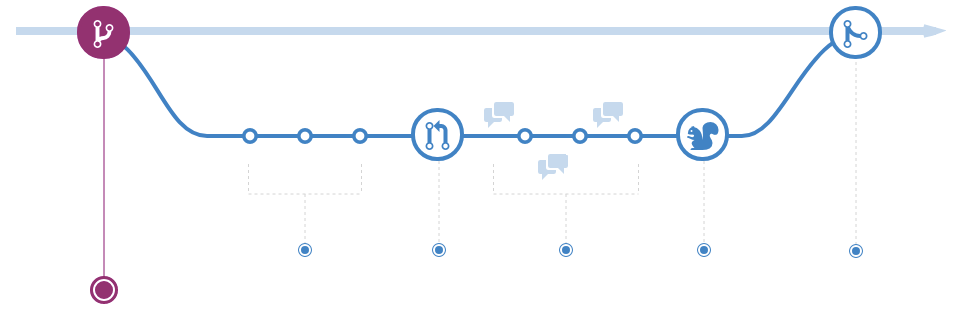
\includegraphics[width=.8\textwidth]{img/git-1.png}
    \end{figure}

    \item New \textbf{versions of software can be produced} in the branch.
    \begin{figure}[!htp]
        \centering
        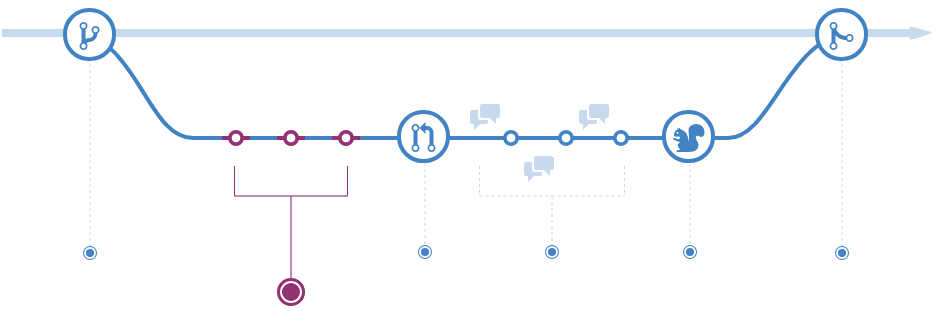
\includegraphics[width=.8\textwidth]{img/git-2.png}
    \end{figure}

    \item When the work is done, we can \textbf{make a pull request}. Then the sub-teams ask the whole team to review the changes and decide whether or not to accept them. The sub-team has already merged any local changes into the server side of the branch.
    \newpage
    \begin{figure}[!htp]
        \centering
        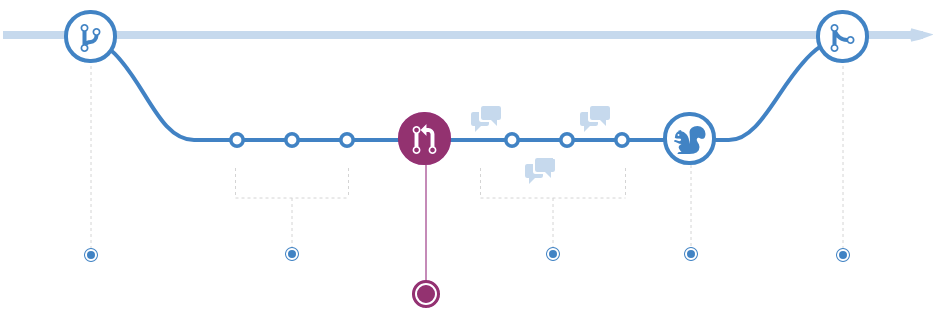
\includegraphics[width=.8\textwidth]{img/git-3.png}
    \end{figure}

    \item A \textbf{discussion starts}, and new versions can be created in the branch during the discussion.
    \begin{figure}[!htp]
        \centering
        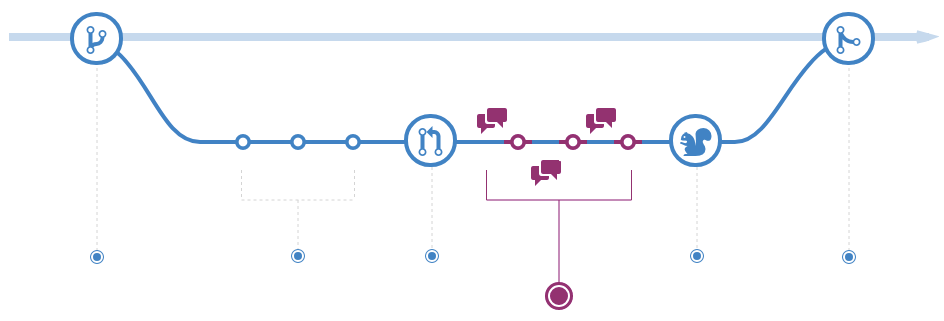
\includegraphics[width=.8\textwidth]{img/git-4.png}
    \end{figure}

    \item Finally, the \textbf{code is deployed and tested}.
    \begin{figure}[!htp]
        \centering
        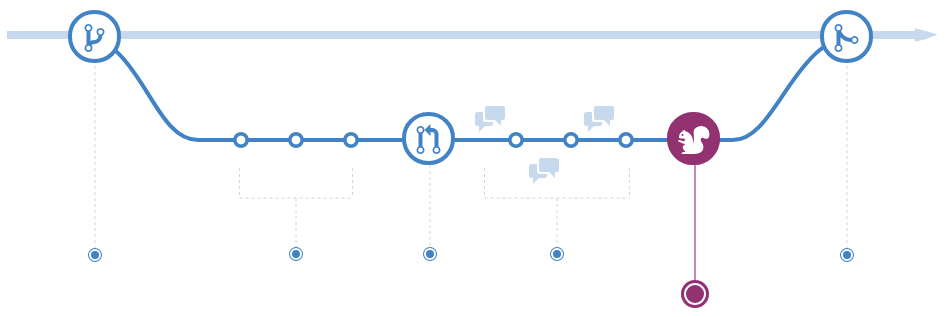
\includegraphics[width=.8\textwidth]{img/git-5.png}
    \end{figure}

    \item And the \textbf{branch is merged into the master}.
    \begin{figure}[!htp]
        \centering
        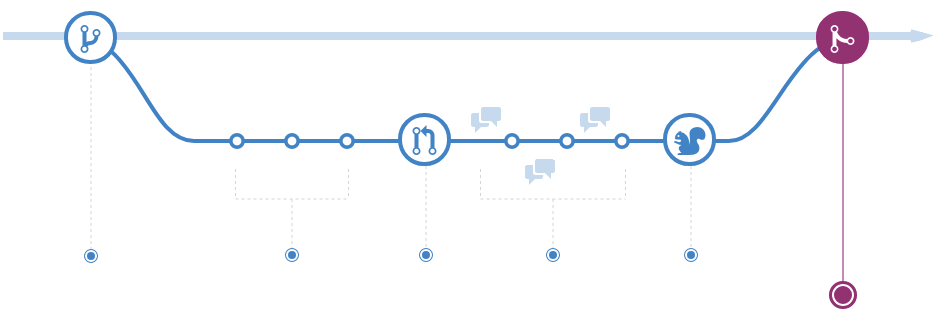
\includegraphics[width=.8\textwidth]{img/git-6.png}
    \end{figure}
\end{enumerate}